\section{Studio dei processi}
Come già detto, un \textbf{processo software} è un insieme di attività atte alla creazione di un software, comprende almeno le quattro attività fondamentali e si sceglie in base al caso di studio. I vantaggi di una sua definizione sono evidenti: garantire uno standard lavorativo e di conseguenza un livello minimo di qualità del prodotto. Esistono numerosi processi software, dai più \textbf{prescrittivi}, caratterizzati da regole e fasi ben definite, ai più \textbf{adattivi}, che privilegiano flessibilità e adattamento ai cambiamenti.\par
Conoscere i modelli di processo è fondamentale per i \textbf{project manager}, poiché è compito loro decidere quale adottare considerando la tipologia del software da progettare. È un tema complesso, perché ha un enorme impatto sulla buona riuscita del progetto. Un secondo motivo per cui è bene conoscere i processi è uscire da quello di bruteforcing, conosciuto anche come \textbf{code and fix}, verosimilmente utilizzato da te fino all'avvento di questa materia. Si tratta di un modus operandi privo di analisi e progettazioni, il cui prodotto si crea esclusivamente per tentativi. È chiaro che non è un metodo adatto per progetti professionali, quindi nelle prossime sezioni analizzeremo le tipologie di processo più usate: a cascata, evolutivi, basati sulla configurazione e integrazione di componenti e agili.

%

\section{Modelli a cascata}
Storicamente, il modello \textbf{Waterfall} è il primo mai utilizzato in ambito di sviluppo software. Mette in cascata i passi tradizionali dello sviluppo di un sistema ed ogni fase produce un \textbf{deliverable}, il quale verrà usato come input di quella successiva, fino al termine del processo. Presenta i seguenti passi: \begin{itemize}
	\item \textbf{Studio della fattibilità}: Valutazione di fattibilità e convenienza in base al tempo e le risorse disponibili. Si stima inoltre il \textbf{return on investment} (ROI), ovvero il guadagno potenziale derivante dall'investimento nello sviluppo del software.
	\item \textbf{Definizione e analisi dei requisiti}: Raccolta delle richieste del cliente. Il deliverable è il \textbf{documento dei requisiti}, il quale fornisce i dettagli in merito alle funzionalità del programma. Può avere definizioni, specifiche o visualizzazioni grafiche.
	\item \textbf{Design del software}: La definizione delle componenti del sistema con le relative relazioni (\textbf{high-level design}) oppure la definizione interna di ogni componente (\textbf{low-level design}). Il deliverable è la specifica del design mediante un \textbf{linguaggio di modellazione unificato} (UML).
	\item \textbf{Implementazione del codice}: La scrittura effettiva del codice insieme al mandatorio unit testing. Ci sono diversi paradigmi di sviluppo, ma il deliverable rimane sempre il codice completo del programma.
	\item \textbf{Verifica del codice}: Il testing del codice con l'eventuale integrazione di soluzioni ai problemi. Il deliverable fornisce i dettagli sui test effettuati insieme ad un report.
	\item \textbf{Mantenimento del codice}: La costante manutenzione del software per la durata del suo ciclo di vita, come l'aggiunta di nuove feature, ottimizzazioni o di adattare il codice alle nuove tecnologie, come l'ultima versione di un sistema operativo.
\end{itemize}
\noindent I pregi dell'uso di questo metodo sono l'enfasi sull'analisi dei requisiti ed il progetto di sistema, perché prima di cominciare ci si assicura di aver determinato correttamente i bisogni del cliente e di averli definiti adeguatamente. Sebbene questo sia un processo solido, allo stesso tempo risulta rigido e monolitico, rendendo difficile contemplare cambiamenti al progetto in corso d'opera.\par
Per far fronte a questo problema di flessibilità sono stati ideati altri modelli ispirati al waterfall che implementano il concetto di feedback e interazioni durante lo sviluppo. Per esempio, nel \textbf{modello a cascata iterativo} si ha la possibilità di ritornare a una fase precedente in base al feedback dato dallo stakeholder, ottenuto di norma fornendo un prototipo. Un'altra variante è il \textbf{modello a V}, che dà molta enfasi al testing, mostrando anche come le loro attività siano collegate a quelle di analisi e progettazione. In questo paradigma, infatti, ogni controllo che non ha esito positivo porta a un rifacimento o modifica della fase associata, per poi riprendere il workflow da quella fase.\par
Sebbene questi due modelli abbiano apportato migliorie al waterfall, è evidente che siano ugualmente poco flessibili agli imprevisti. Nella maggior parte dei casi non è realistico che i requisiti rimangano gli stessi per quelli che potrebbero essere anni di lavoro. Per questo motivo sono stati ideati altri paradigmi di sviluppo software con alla base la possibilità di evolversi in base al feedback del cliente.
\begin{figure}[h]
	\centering
	\subcaptionbox{Modello a cascata}{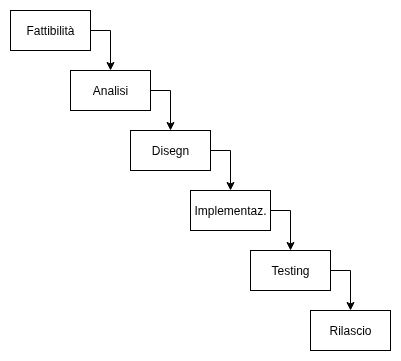
\includegraphics[width=0.45\linewidth]{Images/WaterfallModel.png}}
	\hfill
	\subcaptionbox{Modello a cascata iterativo}{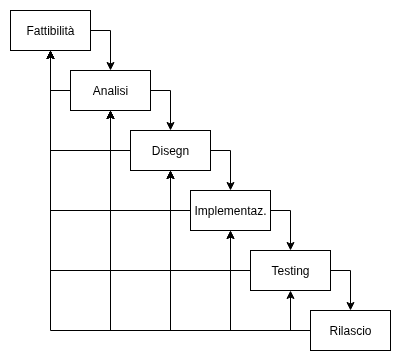
\includegraphics[width=0.45\linewidth]{Images/WaterfallIterationModel.png}}
	\hfill
	\subcaptionbox{Modello a V}{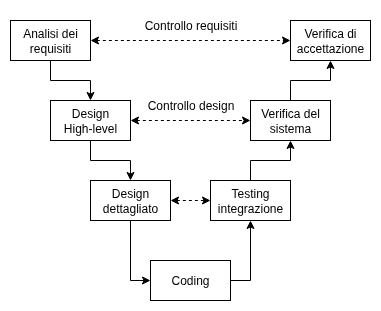
\includegraphics[width=0.45\linewidth]{Images/V-Model.png}}
\end{figure}

%

\section{Modelli evolutivi}



\subsection{Modelli di prototipizzazione}
\subsection{Modelli iterativi-incrementali}

\section{Modello a spirale}
\section{Processo unificato}
\section{Sviluppo basato sui componenti}
\section{Modello trasformazionale}

\section{Metodi agili}

\begin{comment}		
	-- Approcci diversi
	Cerchiamo quindi di sviluppare un'implementazione iniziale, esporla agli utenti e raffinarla release dpopo release, fino ad arrivare alla lista completa di funzionalità.
	Ognuna di queste release può essere utilizzata. Ottimo per potersi gestire con i feedback e correggere problemi con la successiva patch.
	
	- Modelli a prototyping
	Realizza un prototipo funzionante del sistema sul quale validare i requisiti. Se va bene si prosegue, altrimenti lo si rielabora. Il pototipo è ridotto perché ha meno funzionalità
	ed è meno efficiente in termini di prestazioni. Spesso è sviluppato in un linguaggio di alto livello perché accorcia i tempi di lavoro, potendo ottenere feedback quanto prima.
	
	Vantaggi: >Permette di raffinare i requisiti definiti all'inizio e si rilevano velocemente errori di interpretaione.
	Svantaggi: Spesso il prototipo è da buttare, è un problema economico e di stress. Il rischio è di non farlo e così scelte non ideali diventano parte integrante del sistema.
	
	Quindi si protitpizzano le funzionalità su cui il cliente non sembra avere le idee chiare.
	
	- Modelli iterativi-incrementali
	Prevedono di sviluppare più release di cui solo l'ultima è completa. Chiedono di individuare le features per ogni release; dopo la prima si procede in parallelo.
	Nel senso, hai una prima release con le feature base, le successive avranno le funzionalità aggiuntive richieste, distribuendo versioni del software sempre più coplete.
	Sinergia col feedback palese.
	
	Per esempio, per birdArchive:
	- Possibilità di leggere/salvare un archivio
	- Feature per inserimento da CLI
	- Feature per modifica da CLI
	
	Tendenzialmente si implementano prima i requisiti che danno maggior valore al committente, quindi quelle più a lui utili, per le quali ha richiesto il software.
	Un altro approccio potrebbe essere invece di dare tutte e features in una volta, ma parzialmente. Dai parte per parte con ogni release fino al prodotto completo.
	
	Vantaggi: Release sviluppate in base al feedback ed è più semplice prevedere le risorse necessarie allo sviluppo, in quanto più piccole. I problemi vengono anche individuati rpesto
	e c'è anche una risposta rapida al mercato. E' veramente solo usando ill software che si capisce cosa si vuole.
	
	-- Modello a spirale
	Approccio più realistico per sistemi di grandi dimensioni, si evolve insieme alle interazioni continue fra cliente e devs. E' un modello guidato dal rischio.
	Per rischio intendiamo una circostanza potenzialmente avversa in grado di attaccare lo sviluppo e la qualità del sw.
	Ogni scelta, come gli investimenti, comporta un rischio, già la scelta di una tecnologia ne comporta. Prima di scegliere bisogna valutare:
	- gravità delle conseguenze
	- probabilità del verificarsi della circostanza.
	
	Questo modello prevede quattro fasi dove ci continua ad iterare fra loro fino ad arrivare al prodotto definitivo:
	- Planning: determinazione di obiettivi, alternative e vincoli
	- risk analysis: analisi di alternative e identificazione/risoluzione rischi
	- engineering: Sviluppo del prodotto di successivp lovello
	- customer evaluation Revisione dei risultati da parte del committente.
	
	Vantaggi: Adatto a sistemi complessi, ed è un modello guidato dal rischio.
	Svantaggi: Non è universale, necessita poi grandi competenze di valutazione rischi. Richiede un'opportina personalizzazione ed esperienza di utilizzo. Se un rischio rilevante non
	è scoperto o gestito, c'è la possibilità di dover ricominciare da capo. Dipende da quanto è grave la conseguenza.
	
	- Unified Process
	Sviluppo di sistemi a oggetti con notazioni UML per tutto il processo. E' gyuidato dagli use case e incorpora mote idee dal modello a spirale, come lo sviluppo a fase, rilasci
	multipli, con enfasi su ustomer evaluation.
	Ci sono 4 iterazioni con 5 sottofasi per ognuna di loro (nelle slide, è stato troppo veloce):
	- inception: Studio di fattibilità, requisiti essenziali
	- elaboration. comprensione del dominio del problema e definizione architettura
	- construction: design codicfica e testing
	- transition: Messa in esercizio del sistema.
	
	- Component based softEng
	Cerca di minimizzare la scrittura di nuovo codice cercando di riutilizzare componenti già a disposizione piuttosto che scriverne di nuove.
	Esiste uno store o marketplace dei componenti e lo sviluppo inizia con la loro identificazione.
	Fasi: requirements specs -> component analysis -> requirements modifications -> system design with reuse -> dev and integration -> system validation
	Si vanno a controllare le componenti che possono rispondere alle richieste, eventualmente le si cambiano se non è così, poi si fa design e sviluppo, per poi validarlo.
	
	Vantaggi: Scrivo meno codice perché mi affido a roba già scritta. Riduce costi totali e rischi.
	Svantaggi: Inevitabili compromessi perché le componenti non le hai scritte tu, la soluzione sarebbe modificare i requisiti, ma il cliente può essere cagacazzo. Non è sempre facike
	integrare il coice e spesso i componenti usati sono fatti evolvere dalla ditta produttrice senza controllo di chi li usa.
	
	-- Modello trasformazionale
	Guidato da una specifica si arriva all'implementazione. Si tratta di un modello rigoroso e matematico;  si analizzano i requisiti, formalizzarli e li si trasforma per step
	in codice effettivo. Comodo perché posso dimostrare il funzionamento del codice matematicamente.
	
	- Metodi agili
	Prevede di avere meno attenzione sulla documentazione per garantire una migliore flessibilità nell'implementazione del codice. Risulta più importante soddisfare il cliente
	piuttosto che seguire il piano. Ci sono delle fasi abbastanza rapide e brevi:
	- ciclo rapido/consegne frequenti: Ogni ciclo ffronta un solo pezzo e si deve concludere in fretta
	- progettazione semplice: Keep it short and simple, implementa solo le cose necessarie e in modo semplice
	- refactoring: Ristrutturazione continua del codice per renderlo più chiaro
	- meeting di riflessione: Frequenti, giornalieri.
	- tacit/implicit knowledge: Conoscenza nella testa di chi lavora piuttosto che nei documenti (ahimè)
	- Co-location (customer on site): Gli sviluppatori devono lavorare insieme agli utenti, i quali devono essere presenti e disponibili (idealmente).
	
	Approcci molto agili, ma i problemi che portano sono gestionali, legali e di manuytenzione.
	Se perdi un componente del team la knowledge implicita è persa. Gli utenti potrebbero non eessere sempre disponibili.
	Non si sa quando lo sviluppo termina, il contratto non è stipulato, non è scritto da nessuna parte.
	La documentazione è scarsa e a causa di ciò lo sviluppo può evolvere in modo casuale. Disgustosamente casuale.
	
	Generalmente la scelta del metodo:
	- plan-driven se è grosso o critico
	- agile se è una roba più piccolina.
\end{comment}